\documentclass[12pt,fleqn,a4paper]{article}

\usepackage{latexsym}
\usepackage{url}
\usepackage{xspace}
\usepackage{epsfig}
\usepackage{psfrag}
\usepackage{comment}
%\usepackage{a4wide}
\usepackage{marvosym}
\usepackage{amsmath,amsfonts,amssymb,amsthm,latexsym}
\usepackage{graphics,graphicx,color}
\usepackage{fancyhdr}
\usepackage[english]{babel}
\usepackage[latin1]{inputenc}
\usepackage{mathtools}
\textheight 680pt
\textwidth 460pt
\topmargin -40pt
\oddsidemargin 5pt
\evensidemargin 5pt
\parindent 0pt

\pagestyle{fancyplain} \setlength{\headheight}{16pt}
\renewcommand{\sectionmark}[1]{\markright{\thesection\ #1}}
\lhead[\fancyplain{}{\thepage}]
   {\fancyplain{}{\rightmark}}
\rhead[\fancyplain{}{\leftmark}]
   {\fancyplain{}{\thepage}}
\cfoot{}
\renewcommand{\thesection}{\arabic{section}}
\renewcommand{\thesubsection}{\arabic{section}.\arabic{subsection}}

\begin{document}
\begin{titlepage}%Institution
\vspace{2cm}
\centerline{
\large{Department of Computer Sciences}}
\vspace{0.2cm}
\centerline{\large{University of Salzburg}}%Title with one or two Lines(More if wanted)
%\hline
\vspace{2cm}

\centerline{\large{Einf\"{u}hrung Simulation}}
\centerline{SS 13/14}
\vspace{1cm}

\centerline{\huge{Notaufnahme}}
\vspace{1cm}

\vspace{0.4cm}%Date
\centerline{\today}
\vspace{5cm}%Authors

%\hline
\vspace{0.2cm}
Project Members:\\
\centerline{Tobias Auinger, 1220321, auingerto@stud.sbg.ac.at}\\
\centerline{Christian M\"{u}ller, 1123410, mueller110@gmx.net}\\
\centerline{Georgi Potzkov, 0123456, potzkovge@stud.sbg.ac.at}
\vspace {0.8cm}\\

Academic Supervisor: \\
\centerline{asdf}
\centerline{asdf}
\vspace{0.8cm}\\
\clearpage
\end{titlepage}

%%%
%Table of Content
% \setcounter{page}{1}
% \pagenumbering{Roman} %I,II,III... in the TOC
% \tableofcontents

\clearpage
\pagestyle{headings}
\pagenumbering{arabic}  %Better if TOC is variable (more than one page)
\setcounter{page}{1}
\pagenumbering{arabic}  %Better if TOC is variable (more than one page)
\setcounter{page}{1}

\tableofcontents
\newpage

%%%
\section{Einleitung}
In folgender Ausarbeitung sollen  Modell und Ergebnisse der von uns im Rahmen des Proseminars Einf\"{u}hrung Simulation implementierten Projektes besprochen werden.
Ziel des Projektes war es eine auf DesmoJ basierende Simulation einer Notaufnahme zu erstellen. Wir haben uns f\"{u}r den Ansatz der Ereignisorientierten Simulation entschieden dh. Zustands\"{a}nderungen erfolgen stets nur zu bestimmten Ereigniszeitpunkten.

\section{Aufgabe}\label{sec:Aufgabe}
Unsere Aufgabe war es eine Notaufnahme eines Krankenhauses zu simulieren. Die Notaufnahme wird von 2 \"{A}rzten betreut. In dieser Notaufnahme erscheint durschnittlich alle 40 Minuten ein Patient. Der angekommende Patient hat eine Priorit\"{a}t, die seine Dringlichkeit beschreibt. Etwa 20\% der ankommenden Patienten haben die Priorit\"{a}t 3 und m\"{u}ssen so schnell wie m\"{o}glich behandelt werden. Sie sind also akute Notf\"{a}lle. Der Rest, also Patienten mit der Priorit\"{a}t 1, kann warten. Nach einer Behandlung eines Patienten, wird dessen Priorit\"{a}t auf 2 gesetzt. Diese Patienten werden noch einmal f\"{u}r eine Nachbehandlung gebraucht, bevor sie die Notaufnahme endg\"{u}ltig verlassen.
Zu simulieren war ein l\"{a}ngerer Zeitraum, wie etwa 20 Tage. Die Notaufnahme hat dabei immer offen zu sein.
Ebenso war es unsere Aufgabe Erweiterungen zu \"{u}berlegen und zu implementieren.

\section{Erweiterungen}
Wie schon in \ref{sec:Aufgabe} angesprochen, sollten wir ebenfalls ein paar Erweiterungen \"{u}berlegen und implementieren. Um ein bisschen Realit\"{a}tsn\"{a}her zu sein, dachten wir uns, dass dringendere Notf\"{a}lle (Patienten mit Priorit\"{a}t 3) nicht so dringende Patienten (Patitienten mit Priorit\"{a}t 1) verdr\"{a}ngen k\"{o}nnen, da diese eventuell schwerwiegende, also lebensbedrohende, Verletzungen haben k\"{o}nnen.
Desweiteren dachten wir uns, dass akute Notf\"{a}lle auch versterben k\"{o}nnen. Somit sind wir auf den Entschluss gekommen, den Patienten mit der Priorit\"{a}t 3 eine zuf\"{a}llige Restzeit zu geben, in der sie behandelt werden m\"{u}ssen. Werden sie jedoch nicht behandelt, versterben die Patienten und werden dadurch auch aus der Notausnahme gebracht.

\section{Events und Warteschlangen}
\subsection{New Patient Event}
Um einen neuen Patienten zu erzeugen verwenden wir unser New Patient Event. Nun wird eine neue Patient Entit\"{a}t erstellt. Hierbei bekommt der Patient mit einer Warscheinlichkeit von 20% die Priorit\"{a}t 3, sonst bekommt er die Priorit\"{a}t 1. Nun wird ein neues Patient Arrival Event f\"{u}r jenen Patienten erstellt, und ebenso ein New Patient Event erstellt, sodass immer wieder neue Patienten kommen.
%\frametitle{NewPatientEvent Modell}
\begin{center}
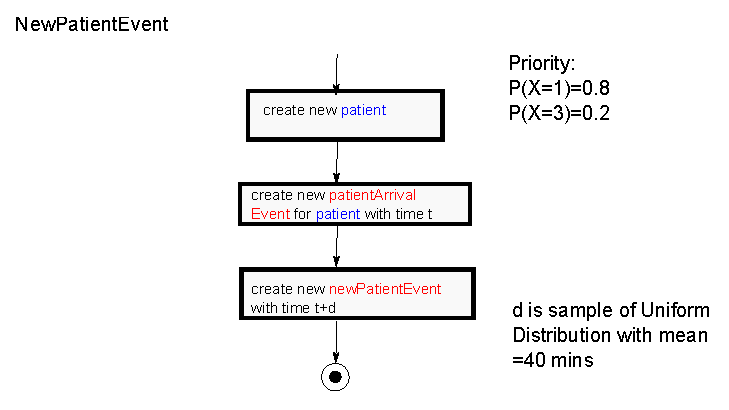
\includegraphics[scale=1]{img/NewPatientEvent}
\end{center}




\subsection{Patient Arrival Event}

%\frametitle{PatientArrivalEvent Modell}
PatientArrivalEvent modelliert die Ankunft eines Patienten. 
Abh\"{a}ngig von der Priorit\"{a}t des Patienten wird dieser in einer der 3 Warteschlangen gegeben. Wurde der Patient im Sinne unserer Erweiterung von einem Patienten mit Priorit\"{a}t 3 abgel\"{o}\ss t dh. wurde seine Behandlung durch einen Priorit\"{a}t 3 abgebrochen, wird dieser in vorne in die Warteschlange seiner Priorit\"{a}t eingereiht. Handelt es sich bei dem Patienten um einen Patienten der Priorit\"{a}t 3 wird f\"{u}r diesen weiter die Zeitpunkt seines Todes bestimmt. (PatientDeathEvent)
Abh\"{a}ngig davon ob ein Doktor frei ist dh. gerade keinen Patienten behandelt oder nicht wird der Patient einem Doktor zugewiesen oder aber er verbleibt in der Warteschlange. 
Handelt es sich beim Patienten um einen Notfall hat dieser auch wenn kein Doktor frei sein sollte durch Abl\"{o}sung eines sich in Behandlung befindlichen Priorit\"{a}t 1 Patienten die M\"{o}glichkeit sofort behandelt zu werden. 


\begin{center}
%    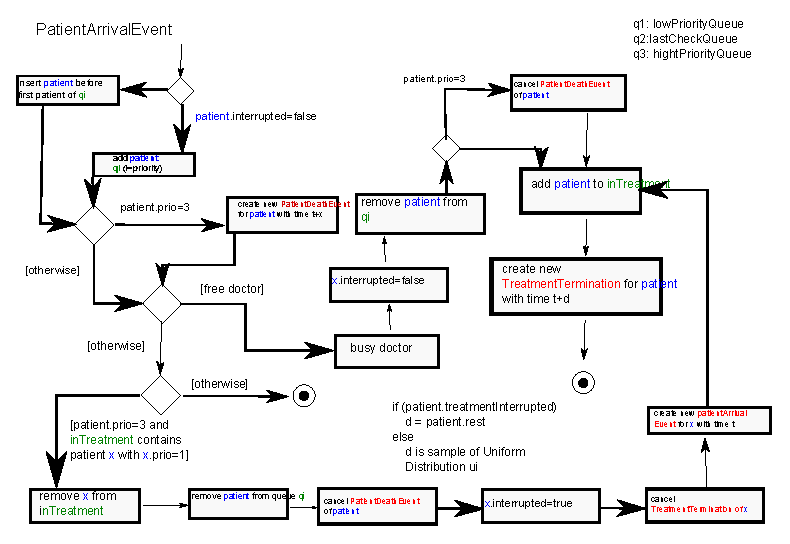
\includegraphics[scale=0.8]{img/PatientArrivalEvent}
\end{center}



\subsection{Treatment Termination Event}
Das Treatment Termination Event ist sowhol auschlaggebend f\"{u}r den weiteren Verlauf in der Notaufnahme des Patienten, als auch f\"{u}r die Dauer seiner Behandlung. Der Patient wird aus der Behandlungswarteschlange genommen. Ist dessen Priorit\"{a}t nicht 2 (sondern 3 oder 1), dann wird seine Priorit\"{a}t auf 2 gesetzt und anschlie\ss end ein Patient Arrival Event f\"{u}r diesen erstellt. Ist jedoch seine Priorit\"{a}t 2, so verl\"{a}sst er die Notaufnahme.
Beinhalten nun alle Warteschlangen der Patienten keine Patienten, so wird der Doktor (der diesen Patienten behandelte) auf verf\"{u}gbar gesetzt, in dem er der Free Doctor Warteschlange hinzugef\"{u}gt wird. Enth\"{a}lt jedoch eine der Patienten Warteschlangen einen Patienten (\"{U}berpr\"{a}fung erfolgt absteigend (3,2,1)),  so wird dieser aus der Warteschlange entfernt und wird von einem Doktor behandelt (Hinzuf\"{u}gen der Treatement Warteschlange). Ebenso wird ein neues Treatement Termination Event f\"{u}r den neuen Patienten mit einer Behandlungszeit erstellt und der Ereignisliste hinzugef\"{u}gt.
Hat dieser neue Patient eine Priorit\"{a}t von 3, so wird sein Patient Death Event, welches den Tod f\"{u}r diesen nicht behandelten akuten Notfall darstellt, abgebrochen.
%\frametitle{TreatmentTermination Modell}
\begin{center}
%    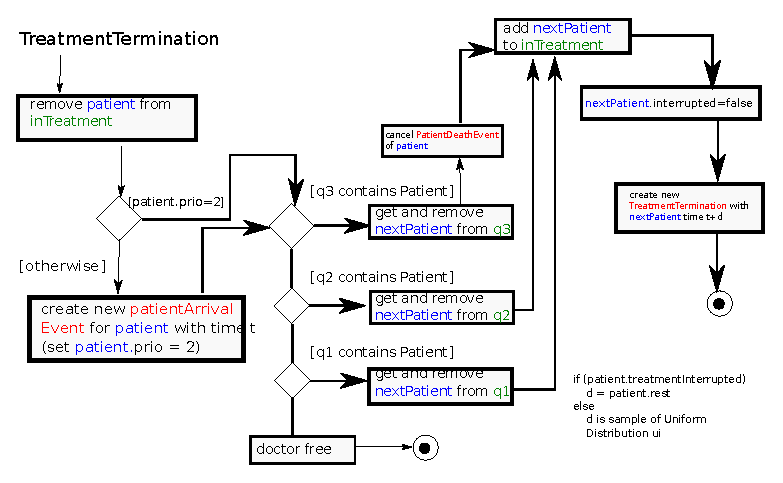
\includegraphics[scale=0.9]{img/TreatmentTermination}
\end{center}



\subsection{Busy/Free Doctor Warteschlangen}
Die Doktoren in unserer Notaufnahme werden mittels zwei Warteschlangen verwaltet. Diese Graphik beschreibt den Statuswechsel der Doktoren.
%\frametitle{Busy/Free Doctor}
\begin{center}
    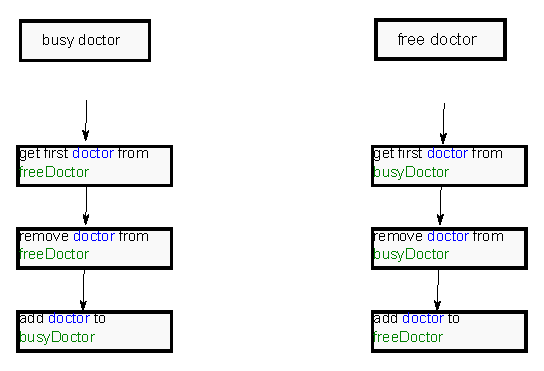
\includegraphics[scale=1]{img/freeDoctor}
\end{center}



\section{Ergebnisse}
Im folgenden sollen die Ergebnisse, welche das Resultat von jeweils hundert Simulationsl\"{a}ufen sind, einer n\"{a}heren Betrachtung unterzogen werden.
Wie in \ref{sec:Aufgabe} beschrieben, war es Teil der Aufgabenstellung die Simulation mit und ohne Initialisierungsphase durchzuf\"{u}hren.
Desweiteren haben wir die Auswirkung  der von uns erdachten Erweiterungen betrachtet und analysiert.





\newpage
%
% end of document
%
\end{document}



